\subsection{x86}

\index{x86!\Instructions!LOOP}
\RU{Для организации циклов в архитектуре x86 есть старая инструкция \LOOP. 
Она проверяет значение регистра \ECX и если оно не 0, делает \glslink{decrement}{декремент} \ECX 
и переход по метке, указанной в операнде. 
Возможно, эта инструкция не слишком удобная, потому что я не видел современных компиляторов, 
которые использовали бы её. Так что если вы видите где-то \LOOP, то с большой вероятностью это 
вручную написанный код на ассемблере.}
\EN{There is a special \LOOP instruction in x86 instruction set for checking the value in register \ECX and 
if it is not 0, to \gls{decrement} \ECX
and pass control flow to the label in the \LOOP operand. 
Probably this instruction is not very convenient, as I never saw any modern compiler emit it automatically.
So, if you see this instruction somewhere in code, it is most likely that this is a manually written piece 
of assembly code.}\\
\\
\RU{Обычно, циклы на \CCpp создаются при помощи \TT{for()}, \TT{while()}, \TT{do/while()}.}
\EN{In \CCpp loops are usually constructed using \TT{for()}, \TT{while()} or \TT{do/while()} statements.}

\RU{Начнем с}\EN{Let's start with} \TT{for()}.
\index{\CLanguageElements!for}

\RU{Это выражение описывает инициализацию, условие, операцию после каждой итерации
(\glslink{increment}{инкремент}/\glslink{decrement}{декремент})
и тело цикла.}
\EN{This statement defines loop initialization (set loop counter to initial value), 
loop condition (is the counter bigger than a limit?), what is done at each iteration (\gls{increment}/\gls{decrement})
and of course loop body.}

\lstinputlisting{patterns/09_loops/simple/loops_1.c.\LANG}

\RU{Примерно так же, генерируемый код и будет состоять из этих четырех частей.}
\EN{The generated code is consisting of four parts as well.}

\RU{Возьмем пример}\EN{Let's start with a simple example}:

\lstinputlisting[label=loops_src]{patterns/09_loops/simple/loops_2.c}

\RU{Имеем в итоге}\EN{Result} (MSVC 2010):

\lstinputlisting[caption=MSVC 2010]{patterns/09_loops/simple/1_MSVC.asm.\LANG}

\RU{В принципе, ничего необычного.}\EN{As we see, nothing special.}

\ifdefined\IncludeGCC
\RU{GCC 4.4.1 выдает примерно такой же код, с небольшой разницей:}
\EN{GCC 4.4.1 emits almost the same code, with one subtle difference:}

\lstinputlisting[caption=GCC 4.4.1]{patterns/09_loops/simple/1_GCC.asm.\LANG}

\RU{Интересно становится, если скомпилируем этот же код при помощи MSVC 2010 с включенной оптимизацией}
\EN{Now let's see what we get with optimization turned on} (\Ox):
\fi

\lstinputlisting[caption=\Optimizing MSVC]{patterns/09_loops/simple/1_MSVC_Ox.asm}

\RU{Здесь происходит следующее: переменную $i$ компилятор не выделяет в локальном стеке, 
а выделяет целый регистр под нее: \ESI. 
Это возможно для маленьких функций, где мало локальных переменных.}
\EN{What happens here is that space for the $i$ variable is not allocated in the local stack anymore,
but uses an individual register for it, \ESI.
This is possible in such small functions where there aren't many local variables.}

\RU{В принципе, всё то же самое, только теперь одна важная особенность: 
\ttf не должна менять значение \ESI. 
Наш компилятор уверен в этом, а если бы и была необходимость использовать регистр \ESI в функции \ttf, 
то её значение сохранялось бы в стеке. Примерно так же как и в нашем листинге: 
обратите внимание на \TT{PUSH ESI/POP ESI} в начале и конце функции.}
\EN{One very important thing is that the \ttf function must not change the value in \ESI.
Our compiler is sure here. 
And if the compiler decides to use the \ESI register in \ttf too, its value would have to be saved 
at the function's prologue and restored at the function's epilogue,
almost like in our listing: please note \TT{PUSH ESI/POP ESI}
at the function start and end.}

\ifdefined\IncludeGCC
\RU{Попробуем GCC 4.4.1 с максимальной оптимизацией (\Othree):}
\EN{Let's try GCC 4.4.1 with maximal optimization turned on (\Othree option):}

\lstinputlisting[caption=\Optimizing GCC 4.4.1]{patterns/09_loops/simple/1_GCC_O3.asm}

\index{Loop unwinding}
\RU{Однако GCC просто \IT{развернул} цикл\footnote{\gls{loop unwinding} в англоязычной литературе}.}
\EN{Huh, GCC just unwound our loop.}

\RU{Делается это в тех случаях, когда итераций не слишком много (как в нашем примере)
и можно немного сэкономить время, убрав все инструкции, обеспечивающие цикл. 
В качестве обратной стороны медали, размер кода увеличился.}
\EN{\Gls{loop unwinding} has an advantage in the cases when there aren't much iterations and 
we could cut some execution time by removing all loop support instructions. 
On the other side, the resulting code is obviously larger.}

\EN{Big unrolled loops are not recommended in modern times, because bigger functions
may require bigger cache footprint}%
\RU{Использовать большие развернутые циклы в наше время не рекомендуется, потому что большие
функции требуют больше кэш-памяти}%
\footnote{
\EN{A very good article about it}\RU{Очень хорошая статья об этом}: \cite{DrepperMemory}.
\EN{Another recommendations about loop unrolling from Intel are here}
\RU{А также о рекомендациях о развернутых циклах от Intel можно прочитать здесь}: 
\cite[3.4.1.7]{IntelOptimization}.}.\\
\\
\RU{Увеличим максимальное значение $i$ в цикле до 100 и попробуем снова. GCC выдает:}
\EN{OK, let's increase the maximum value of the $i$ variable to 100 and try again. GCC does:}

\lstinputlisting[caption=GCC]{patterns/09_loops/simple/2_GCC.asm.\LANG}

\RU{Это уже похоже на то, что сделал MSVC 2010 в режиме оптимизации (\Ox). 
За исключением того, что под переменную $i$ будет выделен регистр \EBX.}
\EN{It is quite similar to what MSVC 2010 with optimization (\Ox) produce, 
with the exception that the \EBX register is allocated for the $i$ variable.}
\RU{GCC уверен, что этот регистр не будет 
модифицироваться внутри \ttf, а если вдруг это и придётся там сделать, то его значение будет сохранено 
в начале функции, прямо как в \main.}
\EN{GCC is sure this register will not be modified inside of the \ttf function, 
and if it will, it will be saved at the function prologue and restored at epilogue, 
just like here in the \main function.}
\fi

\ifdefined\IncludeOlly
\clearpage
\subsection{x86: \olly}
\index{\olly}

\RU{Скомпилируем наш пример в}\EN{Let's compile our example in} MSVC 2010 \RU{с}\EN{with} \Ox \AndENRU \Obzero 
\RU{и загрузим в}\EN{options and load it into} \olly.

\RU{Оказывается,}\EN{It seems that} \olly \RU{может обнаруживать простые циклы и показывать их в квадратных скобках, 
для удобства}\EN{is able to detect simple loops and show them in square brackets, for convenience}:

\begin{figure}[H]
\centering
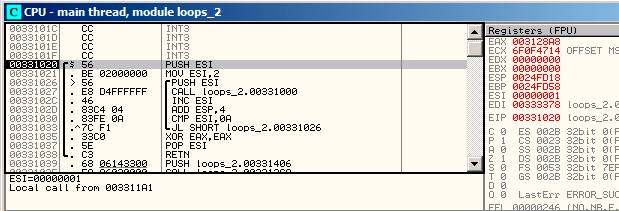
\includegraphics[scale=\FigScale]{patterns/09_loops/simple/olly1.png}
\caption{\olly: \RU{начало \main}\EN{\main begin}}
\label{fig:loops_olly_1}
\end{figure}

\RU{Трассируя}\EN{By tracing} (F8~--- \stepover) \RU{мы видим, как}\EN{we see} \ESI \RU{увеличивается на 1.}
\EN{\glslink{increment}{incrementing}.}
\RU{Например, здесь}\EN{Here, for instance,} $ESI=i=6$:

\begin{figure}[H]
\centering
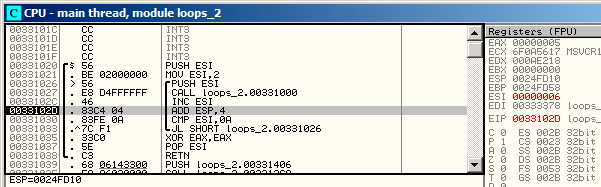
\includegraphics[scale=\FigScale]{patterns/09_loops/simple/olly2.png}
\caption{\olly: \RU{тело цикла только что отработало с}\EN{loop body just executed with} $i=6$}
\label{fig:loops_olly_2}
\end{figure}

9 \RU{это последнее значение цикла}\EN{is the last loop value}.
\RU{Поэтому}\EN{That's why} \JL 
\RU{после \glslink{increment}{инкремента} не срабатывает и функция заканчивается:}
\EN{is not triggering after the \gls{increment}, and the function will finish:}

\begin{figure}[H]
\centering
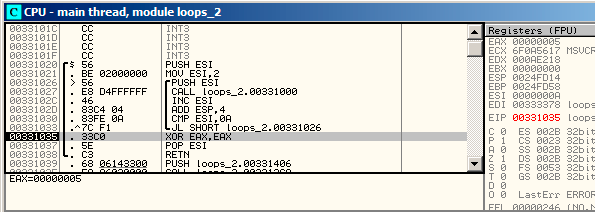
\includegraphics[scale=\FigScale]{patterns/09_loops/simple/olly3.png}
\caption{\olly: $ESI=10$, \RU{конец цикла}\EN{loop end}}
\label{fig:loops_olly_3}
\end{figure}

\subsection{x86: tracer}
\index{tracer}

\RU{Как видно, трассировать вручную цикл в отладчике~--- это не очень удобно.}\EN{As we might see, it is not very
convenient to trace manulally in the debugger.}
\RU{Это одна из причин, почему я писал}\EN{That's one of the reasons I wrote a} \tracer \RU{для себя}%
\EN{for myself}.

\RU{Я открываю скомпилированный пример в}\EN{We open compiled example in} \IDA, 
\RU{нахожу там адрес инструкции}\EN{find the address of the instruction} \TT{PUSH ESI}
(\RU{передающей единственный аргумент в}\EN{passing the sole argument to} \ttf,) 
\RU{а это}\EN{which is} \TT{0x401026} \RU{у меня и запускаю}\EN{for me and we run the} \tracer:

\begin{lstlisting}
tracer.exe -l:loops_2.exe bpx=loops_2.exe!0x00401026
\end{lstlisting}

\RU{Опция }\TT{BPX} 
\RU{просто ставит точку останова по адресу и затем tracer будет выдавать состояние регистров.}
\EN{just sets a breakpoint at the address and tracer will then print the state of the registers.}

\RU{В}\EN{In the} \TT{tracer.log} \RU{после запуска я вижу следующее}\EN{This is what we see}:

\lstinputlisting{patterns/09_loops/simple/tracer.log}

\RU{Видно, как значение}\EN{We see how the value of} \ESI \RU{последовательно изменяется от 2 до 9.}
\EN{register changes from 2 to 9.}

\RU{И даже более того, в \tracer можно собирать значения регистров по всем адресам внутри функции.}
\EN{Even more than that, the \tracer can collect register values for all addresses within the function.}
\RU{Там это называется}\EN{This is called} \IT{trace}\EN{ there}.
\RU{Каждая инструкция трассируется, значения самых интересных регистров запоминаются}\EN{Every instruction
gets traced, all interesting register values are recorded}.
\RU{Затем генерируется .idc-скрипт для \IDA, который добавляет комментарии.}
\EN{Then, an \IDA .idc-script is generated, that adds comments.}
\RU{Итак, в}\EN{So, in the} \IDA \RU{я узнал что адрес}\EN{we've learned that the} \main \RU{это}\EN{function address
is} \TT{0x00401020} \RU{и запускаю}\EN{and we run}:

\begin{lstlisting}
tracer.exe -l:loops_2.exe bpf=loops_2.exe!0x00401020,trace:cc
\end{lstlisting}

\TT{BPF} \RU{означает установить точку останова на функции}\EN{stands for set breakpoint on function}.

\RU{Получаю в итоге скрипты}\EN{As a result, we get the} \TT{loops\_2.exe.idc} \AndENRU 
\TT{loops\_2.exe\_clear.idc}\EN{ scripts}.

\clearpage
\RU{Загружаю}\EN{We load} \TT{loops\_2.exe.idc} \RU{в}\EN{into} \IDA \RU{и увижу следующее}\EN{and see}:

\begin{figure}[H]
\centering
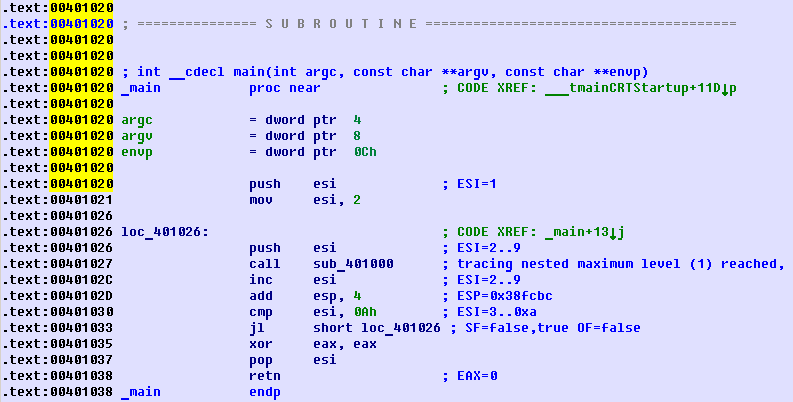
\includegraphics[scale=\FigScale]{patterns/09_loops/simple/IDA_tracer_cc.png}
\caption{\IDA \RU{с загруженным .idc-скриптом}\EN{with .idc-script loaded}}
\label{fig:loops_IDA_tracer}
\end{figure}

\RU{Видно, что}\EN{We see that} \ESI \RU{меняется от 2 до 9 в начале тела цикла, но после 
\glslink{increment}{инкремента} он в пределах [3..0xA]}\EN{can be from 2 to 9 at the start of the loop body,
but from 3 to 0xA (10) after the increment}.
\RU{Видно также, что функция}\EN{We can also see that} \main \RU{заканчивается с 0 в}\EN{is finishing with 0 in} \EAX.

\tracer \RU{также генерирует}\EN{also generates} \TT{loops\_2.exe.txt}, 
\RU{содержащий адреса инструкций, сколько раз была исполнена
каждая и значения регистров}\EN{that contains information about how many times each instruction was executed and
register values}:

\lstinputlisting[caption=loops\_2.exe.txt]{patterns/09_loops/simple/loops_2.exe.txt}
\index{\GrepUsage}
\RU{Так можно использовать grep}\EN{We can use grep here}.

\fi
